%
\RequirePackage{docswitch}
\setjournal{\flag}

\documentclass[\docopts]{\docclass}

% You could define the document class directly
%\documentclass[]{emulateapj}

% 
\usepackage{soul} 
\usepackage{amsmath}
\usepackage{amssymb}
\usepackage{xspace}
\usepackage{xifthen}
\usepackage[dvipsnames,svgnames]{xcolor} 

% General formatting
\newcommand{\ie}{i.e.\xspace}
\newcommand{\eg}{e.g.\xspace}
\newcommand{\etc}{etc.\xspace}
\newcommand{\etal}{et al.\xspace}
\newcommand{\vs}{vs.\xspace}
\newcommand{\super}[1]{\ensuremath{^{\textrm{#1}}}}
\newcommand{\sub}[1]{\ensuremath{_{\textrm{#1}}}}

\newcommand{\FIXME}[1]{{\bf \textcolor{red}{#1}}}
%\newcommand{\FIXME}[1]{{#1}}
\newcommand{\CHECK}[1]{{\bf \textcolor{orange}{#1}}}
%\newcommand{\CHECK}[1]{{#1}}
\newcommand{\COMMENT}[1]{{\it \textcolor{blue}{#1}}}
%\newcommand{\COMMENT}[1]{{#1}}
\newcommand{\NEW}[1]{{\textcolor{blue}{#1}}}
%\newcommand{\NEW}[1]{{#1}}

% Math
\mathchardef\mhyphen="2D
\newcommand{\vect}[1]{\boldsymbol{#1}}
\newcommand{\roughly}{\ensuremath{ {\sim}\,} }
\newcommand{\gtr}{\ensuremath{ {>}\,} }
\newcommand{\less}{\ensuremath{ {<}\,} }
\newlength{\dhatheight}
\newcommand{\doublehat}[1]{%
    \settoheight{\dhatheight}{\ensuremath{\hat{#1}}}%
    \addtolength{\dhatheight}{-0.35ex}%
    \hat{\vphantom{\rule{1pt}{\dhatheight}}%
    \smash{\hat{#1}}}}
\newcommand{\code}[1]{\texttt{#1}\xspace}
\newcommand{\dd}{\ensuremath{\rm d}}
\newcommand{\var}[1]{\ensuremath{#1}\xspace}


% Referencing 
\newcommand{\secref}[1]{Section~\ref{sec:#1}}
\newcommand{\appref}[1]{Appendix~\ref{app:#1}}
\newcommand{\tabref}[1]{Table~\ref{tab:#1}}
\newcommand{\tabrefs}[2]{Tables~\ref{tab:#1} and \ref{tab:#2}}
\newcommand{\figref}[1]{Figure~\ref{fig:#1}}
\newcommand{\figrefs}[2]{Figures~\ref{fig:#1} and \ref{fig:#2}}
\newcommand{\eqnref}[1]{Equation~\eqref{eqn:#1}}

% Astronomy
\newcommand{\LCDM}{\ensuremath{\rm \Lambda CDM}\xspace}
\newcommand{\ra}{{\ensuremath{\alpha_{2000}}}\xspace}
\newcommand{\dec}{{\ensuremath{\delta_{2000}}}\xspace}
\newcommand{\glon}{{\ensuremath{\ell}}\xspace}
\newcommand{\glat}{{\ensuremath{b}}\xspace}

% Units
\newcommand{\unit}[1]{\ensuremath{\mathrm{\,#1}}\xspace}
\newcommand{\Gyr}{\unit{Gyr}}
\newcommand{\MeV}{\unit{MeV}}
\newcommand{\GeV}{\unit{GeV}}
\newcommand{\TeV}{\unit{TeV}}
\newcommand{\degree}{\ensuremath{{}^{\circ}}\xspace}
\newcommand{\mas}{\unit{mas}}
\newcommand{\amin}{\unit{arcmin}}
\newcommand{\asec}{\unit{arcsec}}
\newcommand{\angstrom}{\unit{\AA}}
\newcommand{\um}{\unit{$\mu$m}}
\newcommand{\cm}{\unit{cm}}
\newcommand{\km}{\unit{km}}
\newcommand{\pc}{\unit{pc}}
\newcommand{\kpc}{\unit{kpc}}
\newcommand{\second}{\unit{s}}
\newcommand{\us}{\unit{$\mu$s}}
\newcommand{\photons}{\unit{ph}}
\newcommand{\photon}{\unit{ph}}
\newcommand{\sr}{\unit{sr}}
\newcommand{\Msolar}{\ensuremath{M_\odot}}
\newcommand{\Msun}{\ensuremath{M_\odot}}
\newcommand{\Mstar}{\ensuremath{M_{*}}}
\newcommand{\Lsolar}{\ensuremath{L_\odot}}
\newcommand{\Lsun}{\ensuremath{L_\odot}}
\newcommand{\Lstar}{\ensuremath{L_{*}}}
\newcommand{\Lum}{\ensuremath{ L }\xspace}
\newcommand{\cmcubes}{\ensuremath{\cm^{3}\second^{-1}}\xspace}
\newcommand{\magn}{\unit{mag}}
\newcommand{\mmag}{\unit{mmag}}
\providecommand{\deg}{}
\renewcommand{\deg}{\unit{deg}}
\newcommand{\kms}{{\km\second^{-1}}}
% 


\usepackage[outdir=./]{epstopdf}
\usepackage{graphicx}
\graphicspath{{./}{./figures/}}
\bibliographystyle{apj}
\newcommand{\todo}[1]{\textcolor{magenta}{To do: #1}}
\newcommand{\mrm}[1]{\mathrm{#1}}

%This is a paper and note template for the LSST DESC \citep{Overview,ScienceBook,WhitePaper}.
%Eventually it will be possible to switch between various \LaTeX\xspace styles for internal notes and peer reviewed journals templates.
%The base switch is between \code{aastex.cls} and \code{revtex.cls}; however, facilities are also provided for \code{emulateapj.cls} and \code{mnras.cls}.\footnote{The \code{mnras.cls} class file is a bit odd...}
%Documents can be compiled using the provided \code{Makefile} with several options: \code{make apj}, \code{make apjl}, \code{make prd}, and \code{make mnras}.
%There are some oddities when changing between templates, so please be patient while we try to work these out.

%There are a number of useful \LaTeX\xspace commands predefined in \code{macros.tex}.
%Notice that the section labels are prefixed with \code{sec:} to allow the use of the \verb=\secref= command to reference a section (\ie, \secref{intro}).
%Figures can be referenced with the \verb=\figref= command, which assumes that the figure label is prefixed with \code{fig:}.
%In \figref{example} we show an example figure.
%You'll notice that the actual figure file is found in the \code{figures} directory.
%However, because we have specified this directory in our \verb=\graphicspath= we do not need to explicitly specify the path to the image.

%The \code{macros.tex} package also contains some conventional scientific units like \angstrom, \GeV, \Msun, etc. and some editorial tools for highlighting \FIXME{issues}, \CHECK{text to be checked}, \COMMENT{comments}, and \NEW{new additions}.

%%%%%%%%%%%%%%%%%%%%%%%%
%% Start the Document %%
%%%%%%%%%%%%%%%%%%%%%%%%

\begin{document}

\title{Core Cosmology Library: Precision Cosmological Predictions for LSST}

\maketitlepre

\begin{abstract}

The Core Cosmology Library ({\tt CCL}) provides routines to compute basic cosmological observables with validated numerical accuracy. These routines have been validated to a hereby documented accuracy level against the results of the Code Comparison Project. In the current version, predictions are provided for distances and background quantities, angular auto- and cross-spectra of cosmic shear and clustering and the halo mass function. Fiducial specifications for the expected LSST galaxy distributions and clustering bias are also included, together with a facility to compute redshift distributions for a user-defined photometric redshift model. {\tt CCL} is written in C with a Python interface. In this note, we explain the functionality of the first release ({\tt CCL} v0.1) of the library.

\end{abstract}

% Keywords for paper
%\dockeys{latex: templates, papers: awesome}

\maketitlepost

\newpage
\tableofcontents{}
\newpage

\section{Introduction}
\label{sec:intro}

In preparation for constraining cosmology with the Large Synoptic Survey Telescope (LSST), it is necessary to be able to produce theoretical predictions for the cosmological quantities which will be measured. The Core Cosmology Library\footnote{\url{https://github.com/LSSTDESC/CCL}} ({\tt CCL}) aims to provide, in one library, predictions which are validated to a well-documented numerical accuracy for the purpose of constraining cosmology with LSST. By constructing a cosmology library with LSST in mind, it is possible to ensure that it is flexible, adaptable, and validated for all cases of interest, as well as user-friendly and available for the needs of all working groups.

The Core Cosmology Library is written in C and incorporates the {\tt CLASS} code \cite{class} to provide predictions for the matter power spectrum\footnote{Future versions of the library will incorporate other power-spectrum libraries and methods.}. A Python wrapper is also provided for improved ease of use.

This note describes how to install {\tt CCL} (Section \ref{sec:install}), its functionality (Section \ref{sec:func}), the relevant unit tests (Section \ref{sec:tests}), the default configuration (Section \ref{sec:default}), directions for finding a {\tt CCL} example (Section \ref{sec:example}), the Python wrapper (Section \ref{sec:python}), future plans (Section \ref{sec:future}), means to contact the developers (Section \ref{sec:feedback}) and the license under which {\tt CCL} is released (Section \ref{sec:license}).


\section{Installation}
\label{sec:install}

\subsection{Dependencies}

\begin{itemize}
\item GNU Scientific Library {\tt GSL}\footnote{\url{https://www.gnu.org/software/gsl/}}, {\tt GSL-2.1} or higher
\item Simplified Wrapper and Interface Generator {\tt SWIG}\footnote{\url{http://www.swig.org/}}
\item {\tt FFTlog}\footnote{\url{http://casa.colorado.edu/~ajsh/FFTLog/}} is provided within {\tt CCL} with minor modifications
\item {\tt SWIG} is not needed to run {\tt CCL}, but if you are developing new features, you will need {\tt SWIG}.
\item A version of {\tt Angpow} \citep{2017arXiv170103592C} is also incorporated within {\tt CCL}.
\end{itemize}

\subsection{Installation Procedure}

{\tt CCL} can be installed through an {\tt autotools}-generated configuration file. UNIX users should be familiar with the process: navigate to the directory containing the library and type
\begin{verbatim}
 $ ./configure
 $ make
 $ make install
\end{verbatim}
(You may need to pre-append {\tt sudo} to the last command, depending on your default privileges.) Users without admin privileges can install the library in a user-defined directory (e.g. {\tt /home/desc$\_$fan/}) by running
\begin{verbatim}
 $ ./configure --prefix=/home/desc_fan
 $ make
 $ make install
\end{verbatim}
This will create two directories (if not present already): {\tt /home/desc$\_$fan/include} and {\tt /home/desc$\_$fan/lib} where the header and lib files will be placed after running {\tt make install}. CCL has been successfully installed in different Linux and Mac OS X systems\footnote{We know of one case with Mac OS where libtools had the ``lock'' function set to ``yes'' and this caused the installation to stall. However, this is very rare. If this happens, after the {\tt configure} step, edit libtool to set the ``lock'' to ``no''.}.

After installing the C library you can make sure it is running as it should by typing {\tt make check}, which will run the unit tests described in Section \ref{sec:tests}. You are now ready to install the Python wrapper following the steps described in Section \ref{sec:python}.

There exists also the possibility of installing both the C library and the Python wrapper together by running
\begin{verbatim}
 $ python setup.py install --prefix=/home/desc_fan
\end{verbatim}
This will perform automatically the aforementioned steps to install the C library and will also install the Python library in {\tt /home/desc$\_$fan/lib/python2.7/site-packages}. You might need to add this path to your environment variable {\tt \$PYTHONPATH} to be able to use it. In the near future the package is planned to be {\tt pip} installable.

\todo{We need an update on the pip installation before Public Release}

Once installed you can check the installation status by typing
\begin{verbatim}
 $ python setup.py test
\end{verbatim}

This will run the embedded unit tests. Using this last method to install the Python library allows you to uninstall it just by running
\begin{verbatim}
 $ python setup.py uninstall
\end{verbatim}
 
\subsection{Compiling against an external version of CLASS}

{\tt CCL} has a built-in version of {\tt CLASS} that is used to calculate power spectra and other cosmological functions. This is compiled by default. Optionally, you can also link {\tt CCL} against an external version of {\tt CLASS}. This section useful if you want to use a modified version of {\tt CLASS}, or a different or more up-to-date version of the standard {\tt CLASS}. For example, we have sucessfully compiled and ran {\tt CCL} with {\tt hiCLASS} \citep{hiclass} for Horndeski models.

To compile {\tt CCL} with an external version of {\tt CLASS}, you must first prepare the external copy so that it can be linked as a shared library. By default, the {\tt CLASS} build tools create a static library. After compiling {\tt CLASS} in the usual way (by running {\tt make}), look for a static library file called {\tt libclass.a} that should have been placed in the root source directory. Then, run the following command from that directory (Linux only):
\begin{verbatim}
 $ gcc -shared -o libclass.so -Wl,--whole-archive libclass.a \
                              -Wl,--no-whole-archive -lgomp
\end{verbatim}
This should create a new shared library, {\tt libclass.so}, in the same directory. (N.B. The {\tt -lgomp} flag has to appear at the end of the command; otherwise the linker can fail.) If you are running Mac OS X, use the following command instead:
\begin{verbatim}
 $ gcc -fpic -shared -o libclass.dylib -Wl,-all_load libclass.a -Wl,-noall_load
\end{verbatim}

Next, change to the root {\tt CCL} directory and run {\tt make clean} if you have previously run the compilation process. Then, set the {\tt CLASSDIR} environment variable to point to the directory containing {\tt libclass.so}:
\begin{verbatim}
export CLASSDIR=/path/to/external/class
\end{verbatim}
Then, run {\tt ./configure} and compile and install {\tt CCL} as usual. The {\tt CCL} build tools should take care of linking to the external version of {\tt CLASS}.

Once compilation has finished, run {\tt make check} to make sure everything is working correctly. Remember to add the external {\tt CLASS} library directory to your system library path, using either {\tt export LD\_LIBRARY\_PATH=/path/to/external/class} (Linux) or {\tt export DYLD\_FALLBACK\_LIBRARY\_PATH=/path/to/external/class} (Mac). The system must be able to find both the {\tt CCL} and {\tt CLASS} libraries; it is not enough to only add {\tt CCL} to the library path.

\subsection{Creating a Docker Image}
{\tt CCL} supports the use of the Docker project for the deployment of applications inside software containers. The included Dockerfile allows for quick creation of an image file that will allow for easy realization of virtual machines that require no additional dependencies beyond the Docker software. The Docker website\footnote{\url{https://www.docker.com}} details the installation process for most common operating systems.

With Docker is installed, creating an image is relatively straightforward:
\begin{verbatim}
docker build -t ccl .
\end{verbatim}
This will begin the process of creating the image file for {\tt CCL} locally. This Dockerfile contains all installed C libraries in {\tt CCL} as well as the Python wrapper. It currently utilizes {\tt python:2.7} as a base image and supports both ipython and Jupyter notebook. The virtualization process should have minimum impact on performance.

The resulting Docker image has two primary functionalities. The first is a command that will open a Jupyter notebook tied to a port connection on your local machine. This can be utilized with the following command on run:
\begin{verbatim}
docker run -p 8888:8888 ccl
\end{verbatim}
This Jupyter notebook can be accessed on a browser of your choice at {\tt localhost:8888}. The second possible run is to access the bash itself, which can be done with the command:
\begin{verbatim}
docker run -it ccl bash
\end{verbatim}
This will allow for full access to the virtual machine for installation of any additional desired dependencies.

\section{Functionality}
\label{sec:func}

\subsection{Supported cosmological models}


\label{sec:cosmologies}
Ultimately, CCL will aim to incorporate theoretical predictions for all cosmological models of interest to LSST. Currently, the following families of models are supported:
\begin{itemize}
 \item Flat, vanilla $\Lambda$CDM 
 \item wCDM and the CPL model ($w_0+w_a$)
 \item Non-zero curvature ($K$)
 \item All the above plus an arbitrary, user-defined, modified growth function (see description in Section \ref{sec:growth})
  \item Relativistic neutrinos and / or a single massive neutrino or multiple equal-mass massive neutrinos
\end{itemize}

Not all functionalities are available for all models. For a reference of what predictions are available for each model, see Table \ref{tab:cosmo}.

The first step to use CCL is to generate a {\tt ccl$\_$cosmology} structure, containing all of the information required to compute cosmological observables. A {\tt ccl$\_$cosmology} structure is generated using the information from a {\tt ccl$\_$parameters} object and a {\tt ccl$\_$configuration} object.

\begin{table}
  \begin{center}
  \caption{Cosmologies implemented in CCL. \label{tab:cosmo}}
  \begin{tabular}{lccccccc}
\hline\hline
Observable/Model & flat $\Lambda$CDM & $\Lambda$CDM+$K$ &  $\Lambda$CDM+$\nu$ & $w$CDM & $w_0+w_a$ & $w_0+w_a+\nu+K$ & MG \\[3pt] 
\hline
Distances & \checkmark & \checkmark & \checkmark & \checkmark & \checkmark & \checkmark & $-$ \\
Growth  & \checkmark & \checkmark & \checkmark & \checkmark & \checkmark & \checkmark  & \checkmark  \\
$P_m(k,z)$ & \checkmark & \checkmark  & \checkmark  & \checkmark & \checkmark & \checkmark & $X$\\
Halo Mass Function & \checkmark & \checkmark & $X$ & \checkmark & \checkmark & $X$ & $X$\\
$C_l$ & \checkmark & \checkmark & \checkmark & \checkmark & \checkmark & \checkmark & (growth only) \\
%Correlation functions & & & & & \\
\hline\hline
\end{tabular}
\end{center}
\end{table}


{\tt ccl$\_$parameters} objects contain information about the cosmological parameters, and are initialized using one of the following routines (the full syntax for each function can be found in the header file {\tt ccl$\_$core.h}):
\begin{itemize}
 \item {\tt ccl$\_$parameters$\_$create(double Omega$\_$c, double Omega$\_$b, double Omega$\_$k, double N\_nu\_rel, double N\_nu\_mass, double mnu, double w0, double wa, double h, double norm$\_$pk, double n$\_$s,int nz$\_$mgrowth,double *zarr$\_$mgrowth,double *dfarr$\_$mgrowth, int *status)}: general {\tt ccl$\_$parameters} constructor supporting all the models described above.
 \item {\tt ccl$\_$parameters$\_$create$\_$flat$\_$lcdm(...)}: particular constructor for flat $\Lambda$CDM cosmologies.
 \item {\tt ccl$\_$parameters$\_$create$\_$flat$\_$wcdm(...)}: constant $w$ cosmologies.
 \item {\tt ccl$\_$parameters$\_$create$\_$flat$\_$wacdm(...)}: $w_0+w_a$.
 \item {\tt ccl$\_$parameters$\_$create$\_$lcdm(...)}: curved $\Lambda$CDM cosmologies.
\end{itemize}
The argument ${\tt norm\_pk}$ can be passed the power spectrum normalization parameterized by $\sigma_8$ or $A_\mathrm{s}$, {\tt ccl$\_$parameters$\_$create} switches to $\sigma_8$ normalization if ${\tt norm\_pk} > 1.e-5$, and to $A_{\mathrm s}$ normalization otherwise.

To include neutrinos (massive or massless), the suffix `{\tt $\_$nu}' may be appended to the latter four {\tt ccl$\_$configuration} objects above (for example: {\tt ccl$\_$parameters$\_$create$\_$lcdm$\_$nu(...)}). Utilizing the corresponding {\tt ccl$\_$configuration} object without this {\tt $\_$nu} suffix will set the contribution from both massless and massive neutrinos to zero. In the case of non-zero massive neutrinos, it may be desirable to set {\tt N\_nu\_rel} such that $N_{\rm eff}=3.046$ in the early universe. In agreement with {\tt CLASS}, when using the default value of $T_{\rm NCDM}$ as described in section \ref{sec:distances} below, {\tt N\_nu\_rel} can be set to 2.0328, 1.0196, and 0.00641 for 1, 2 and 3 massive neutrinos respectively to achieve this.

{\tt ccl$\_$configuration} objects contain information about the prescriptions to be used to compute transfer functions, power spectra, mass functions, etc. A default {\tt ccl$\_$configuration} object is made readily available as {\tt default$\_$config}, for which transfer functions are computed with CLASS, the HaloFit prediction is used for the matter power spectrum and a number of prescriptions can be used to compute the halo mass function.

After initializing an instance of {\tt ccl$\_$parameters} and {\tt ccl$\_$configuration}, the function {\tt ccl$\_$cosmology$\_$create(ccl$\_$parameters,ccl$\_$configuration)} returns a pointer to a {\tt ccl$\_$cosmology} structure, which you will need to pass around to every CCL function.

Directions to an example of {\tt CCL} script are provided in Section \ref{sec:example}. The {\tt README} file has additional extensive documentation for the example run and also regarding the installation.

\subsection{Distances}
\label{sec:distances}

\todo{Add distance modulus.}

The routines described in this subsection are implemented in {\tt ccl$\_$background.c}.

The Hubble parameter is calculated via
%
\begin{align}\label{eq:Ha}
\frac{H(a)}{H_0} &= a^{-3/2}\Big(\Omega_{M,0}+\Omega_{\Lambda,0} a^{-3(w_0+w_a)}
    \exp[3 w_a (a-1)]+\Omega_{K,0} a \nonumber \\ &+(\Omega_{g,0} + \Omega_{\nu, {\rm rel}}) a^{-1} + \Omega_{\nu, {\rm m}}(a)a^3\Big)^{\frac{1}{2}}.
\end{align}

The radial comoving distance is calculated via a numerical integral
\begin{equation}
 \chi(a)= c \int_a^1 \frac{da'}{a'^2 H(a')}.
\end{equation}
The transverse comoving distance is computed in terms of the radial comoving distance as:
\begin{equation}\label{eq:angdist}
 r(\chi)=\left\{\begin{array}{cc}
                 k^{-1/2}\sin(k^{1/2}\chi) & k>0\\
                 \chi & k=0\\
                 |k|^{-1/2}\sinh(|k|^{1/2}\chi) & k<0\\
                \end{array}\right.
\end{equation}
The usual angular diameter distance is $d_A=a\,r(a)$, and the luminosity distance is
$d_L=r(a)/a$.

CCL also contains capability to compute $a(\chi)$ (i.e. the inverse of $\chi(a)$).


\subsection{Density parameter functions}
\label{subsec:densityparam}

The routines described in this subsection are implemented in {\tt ccl$\_$background.c}.

The density parameter functions $\Omega_X(a)$ are calculated for six components:
\begin{itemize}
\item matter density parameter $\Omega_M(a) = \Omega_{M,0} H_0^2 / (a^3 H^2(a) )$,
\item dark energy density parameter $\Omega_\Lambda(a) = \Omega_{\Lambda,0} H_0^2 / H^2(a)$,
\item radiation density parameter $\Omega_g(a) = \Omega_{g,0} H_0^2 / (a^4 H^2(a) )$,
\item curvature density parameter $\Omega_K(a) = \Omega_{K,0} H_0^2 / (a^2 H^2(a) )$,
\item massless neutrino density parameter $\Omega_{\nu, {\rm rel}}(a) = \Omega_{\nu, {\rm rel},0} H_0^2 / (a^4 H^2(a) )$,
\item massive neutrino density parameter $\Omega_{\nu, {\rm m}}(a)$,
\end{itemize}
using the Hubble parameter defined in equation~\ref{eq:Ha}.

For massive neutrinos, $\Omega_{\nu, {\rm m}}(a)$ is calculated by calling a set of functions contained in {\tt ccl\_neutrinos.c}. First, we assume that the mass of one neutrino is equal to $m_{\nu}^{\rm tot} / N_{\rm m}^{\nu}$ (recalling that we assume a single massive neutrino or equal-mass neutrinos). We then compute a quantity called the effective temperature:
\begin{equation}
T_{\nu}^{\rm eff} = T_{\rm CMB} T_{\rm NCDM}.
\label{Tnueff}
\end{equation}
$T_{\rm NCDM}$ here is used to explicitly set the value of $m_{\nu} / \Omega_{\nu}^0$. We choose a default value of $T_{\rm NCDM} = 0.71611$, which corresponds to $m_{\nu} / \Omega_{\nu}^0 = 93.14$ eV, to agree with the default value set by {\tt CLASS}. We define 
\begin{equation}
\mu = \frac{m_{\nu}^{\rm tot}a}{N_{\rm m}^\nu T_{\nu}^{\rm eff}}
\label{mnuOT}
\end{equation}
in units such that $\mu$ is dimensionless. We then conduct the phase-space integral required to get the neutrino density, and multiply by appropriate factors to obtain $\Omega_{\nu, {\rm m}}(a)$:
\begin{equation}
\Omega_{\nu, {\rm m}}(a) = N_{\rm m}^\nu \frac{8 \pi^2(\pi k_b )^3 k_b}{15(c h_{\rm P})^3} \frac{8 \pi G}{3h^2c^2} \left(\frac{T_{\nu}^{\rm eff}}{a}\right)^4 \left(\frac{7}{8}\int_0^{x_{\rm max}} dx \, x^2 \frac{\sqrt{x^2 + \mu^2}}{\exp(x) + 1}\right)
\label{Omnu}
\end{equation}
where $h_{\rm P}$ is Planck's constant and $h$ is $H_0/100$ with $H_0$ in units of km / s / Mpc. $x_{\rm max}$ is set to 1000. The final bracketed term which includes the phase-space integral can be simplified in the limit where $\mu$ is very large or very small: for small $\mu$, it is set to $\frac{7}{8}$, and for large $\mu$, it becomes $0.2776566337\mu$.\todo{Do we need this many digits?}



\subsection{Growth function}
\label{sec:growth}

The routines described in this subsection are implemented in {\tt ccl$\_$background.c}.
To compute the growth function, $D(a)$, the growth factor of matter perturbations, {\tt CCL} solves the following differential equation:
\begin{equation}
  \frac{d}{da}\left(a^3H(a)\frac{dD}{da}\right)=\frac{3}{2}\Omega_M(a)aH(a)D.
\end{equation}

In doing this, {\tt CCL} simultaneously computes the so-called growth rate $f(a)$, defined as:
\begin{equation}
  f(a)=\frac{d\ln D}{d\ln a}.
\end{equation}
CCL provides different functions that return the growth normalized to $D(a=1)=1$ and to $D(a\ll1)\rightarrow a$.

Note that the above is strictly valid only for a Universe containing just dust-like components. A scale-independent growth rate is, for example, ill-defined in the presence of massive neutrinos.

Currently CCL allows for an alternative cosmological model defined by a regular background $(w_0+w_a)$CDM (with arbitrary $k$) as well as a user-defined $\Delta f(a)$, such that the true growth rate in this model is given by $f(a)=f_0(a)+\Delta f(a)$, where $f_0(a)$ is the growth rate in the background model. Note that this model is only consistently implemented with regards to the computation of the linear growth factor and growth rates (which will also scale the linear power spectrum), however all other CCL functions (including the non-linear power spectrum) will ignore these modifications. This model, and the interpretation of the predictions given by CCL should therefore be used with care.

\subsection{Matter power spectrum}
\label{sec:power}

There are several options for obtaining the matter power spectrum in {\tt CCL}.
The routines described in this subsection are implemented in {\tt ccl$\_$power.c}.

\subsubsection{BBKS}
CCL implements the analytical BBKS approximation to the transfer function \citep{BBKS}, given by
\begin{equation}
T(q\equiv k/\Gamma h {\rm Mpc}^{-1}) = \frac{\ln[1+2.34q]}{2.34q}[1+3.89q+(16.2q)^2+(5.47q)^3+(6.71q)^4]^{-0.25}
\end{equation}
where $\Gamma = \Omega_m h$.
The power spectrum is related to the transfer function by $\Delta(k)\propto T^2(k)k^{3+n}$ and $\Delta^2(k)\propto k^3P(k)$. The normalization of the power spectrum is achieved at $z=0$ by setting $\sigma_8$ to its value today.
The BBKS power spectrum option is primarily used as a precisely defined input for testing the numerical accuracy of {\tt CCL} routines (as described in Sect.~\ref{sec:tests}), and it is not recommended for other uses.

\subsubsection{CLASS}
Secondly, there is the option to call the {\tt CLASS} software \citep{class} within {\tt CCL} to obtain either linear or nonlinear matter power spectra at given redshifts. For speed, the linear power spectrum is obtained at redshift $z=0$ and re-scaled to a different redshift using the growth function. In the case of the nonlinear matter power spectrum, upon setting up the cosmology object, we construct a bi-dimensional spline in $k$ and the scale-factor which is then called by the relevant routines to obtain the matter power spectrum at the desired wavenumber and redshift. The relevant routines can be found within {\tt ccl$\_$power.c}. Currently CLASS computes the non-linear power spectrum using the HaloFit prescription of \cite{CLASS_halofit}.

\subsubsection{Nonlinear low and high wavenumber extrapolation}
\label{sec:NLextrapol}

\todo{This section needs careful checking, many things have changed here.}

The computation of the power spectrum from {\tt CLASS} can be significantly sped up by extrapolating in the range $k>${\tt K$\_$MAX$\_$SPLINE} and $k<${\tt K$\_$MIN}. In this section, we describe the implementation of the extrapolation and the accuracy attained.

We describe first the extrapolation at high wavenumbers. The introduction of the parameter {\tt K$\_$MAX$\_$SPLINE} allows us to spline the matter power spectrum within the {\tt cosmo} structure up to that value of $k$ (in units of $1/$Mpc). A separate {\tt K$\_$MAX} parameter sets the limit for evaluation of the matter power spectrum. The range between {\tt K$\_$MAX$\_$SPLINE}$<k<${\tt K$\_$MAX} is evaluated by performing a second order Taylor expansion within the static routine {\tt ccl$\_$power$\_$extrapol$\_$highk}.

First, we compute the first and second derivative of the $\ln P(k,z)$ at $k_0={\rm \tt K\_MAX}-2\Delta\ln k$ by computing the numerical derivatives by finite differences using GSL. We then apply a second order Taylor expansion to extrapolate the matter power spectrum to $k>${\tt K$\_$MAX$\_$SPLINE}. The Taylor expansion gives
%
\begin{equation}
  \ln P(k,z) \simeq \ln P(k_0,z) + \frac{d\ln P}{d\ln k}(\ln k_0,z) (\ln k-\ln k_0)  + \frac{1}{2}  \frac{d^2\ln P}{d\ln k^2}(\ln k_0,z) (\ln k-\ln k_0)^2.
  \label{eq:NLPSTaylor}
\end{equation}

The results of this approximation are shown in Figure \ref{fig:NLextrapol} for redshifts $z=0$ and $z=3$ \todo{This figure needs to be updated}. We compare the nonlinear matter power spectrum at $z=0$ computed with the previously described approximation, to the matter power spectrum obtained by directly evaluating {\tt CLASS} at the desired $k$ value. (The benchmark in reality uses a value of {\tt K$\_$MAX$\_$SPLINE}$=10^3$/Mpc, well beyond our range of application.) We find that for typical values of  $\Delta \ln k$ is $10^{-2}$ and {\tt K$\_$MAX$\_$SPLINE}$=50$/Mpc has converged to an accuracy that surpasses the expected impact of baryonic effects on the matter power spectrum at $k>10/$Mpc. (For a plot showing the impact of baryons on the matter power spectrum, see \citealt{Schneider15}.) The lower {\tt K$\_$MAX$\_$SPLINE} is, the faster {\tt CCL} will run. The optimum choice of {\tt K$\_$MAX$\_$SPLINE} is left to the user for their particular application. 

We adopt a similar approach to extrapolate the power spectrum at small scales. In this case, the power spectrum below {\tt K$\_$MIN} is obtained by a power-law extrapolation with index $n_s$:
\begin{equation}
  \log P(k<{\tt K\_MIN},z) = \log P({\tt K\_MIN},z) + n_s (\log k-\log{\tt K\_MIN})
\end{equation}

\todo{Explain choice of default values for {\tt K\_MIN}.}

%------------------------
\begin{figure*}
\centering
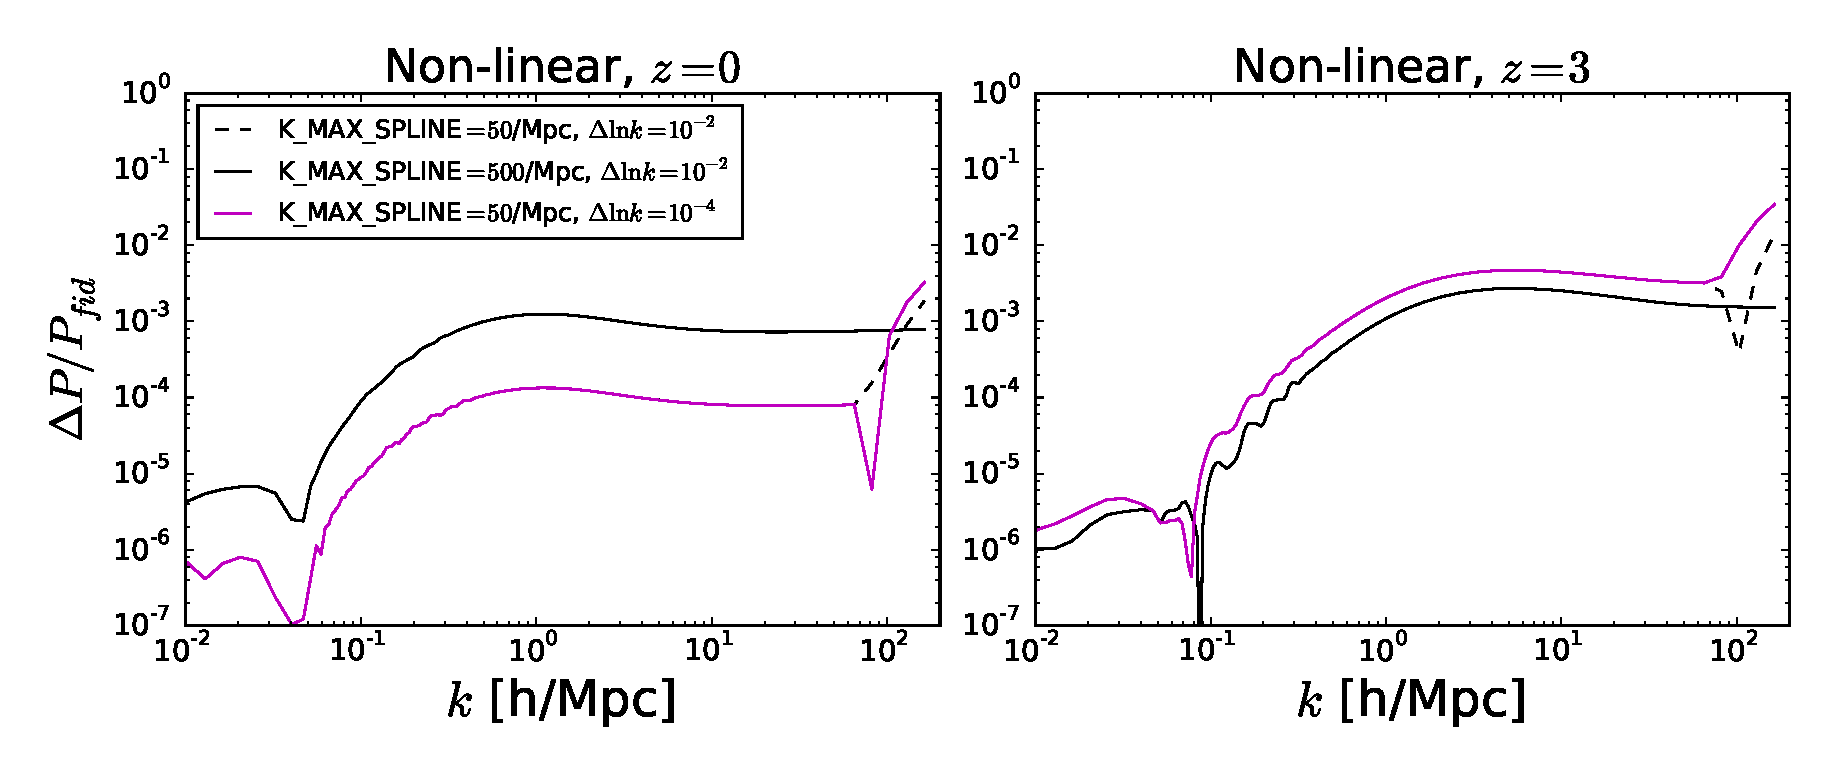
\includegraphics[width=0.45\textwidth]{PS_converge_nonlin.eps}
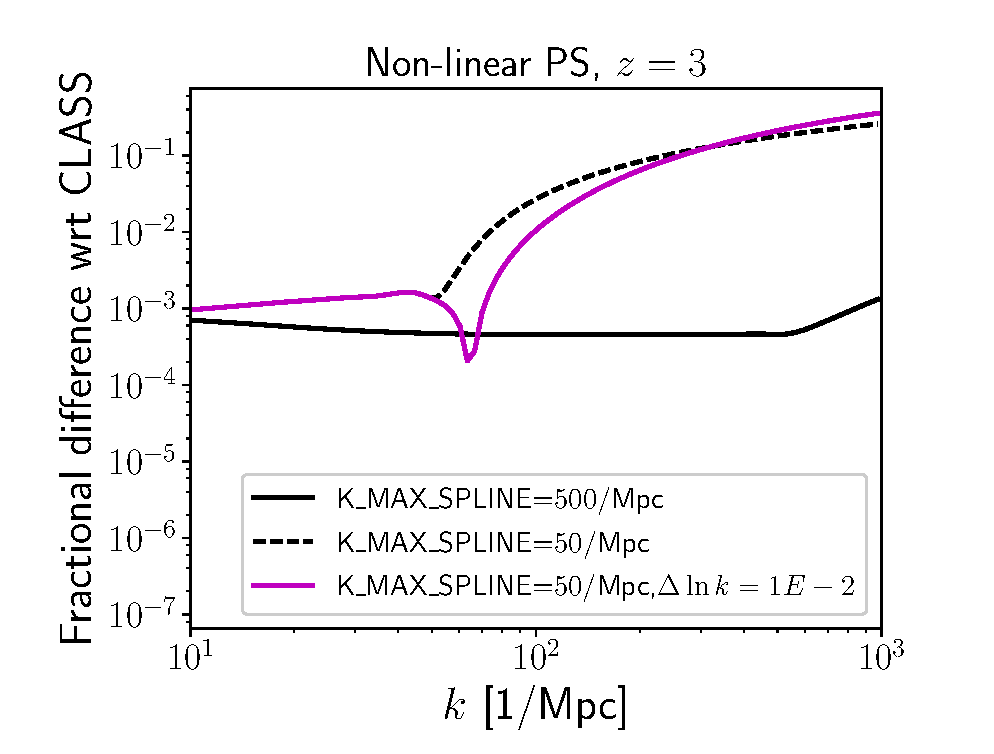
\includegraphics[width=0.45\textwidth]{PS_converge_nonlin_z3.eps}
\caption{The relative error produced by splining the nonlinear matter power spectrum up to {\tt K$\_$MAX$\_$SPLINE} and extrapolating beyond this value with a second order Taylor expansion the natural logarithm of the matter power spectrum. The left panel shows the results at $z=0$. The right panel shows the results at $z=3$. The fiducial parameters adopted are those corresponding to the magenta curve.}
\label{fig:NLextrapol}
\end{figure*}
%------------------------

\paragraph{Linear extrapolation}
\label{sec:Lextrapol}

With the implementation described in the previous section, the power spectrum splines are initialized up to {\tt K$\_$MAX$\_$SPLINE}. This is also true for the linear matter power spectrum, which is used within {\tt CCL} in particular to obtain $\sigma_8$. We have tested here how the procedure described in the previous section affects the convergence of the linear matter power spectrum. We compare the fiducial {\tt CCL} output to the case where we set {\tt K$\_$MAX$\_$SPLINE}$=10^3/$Mpc. The result is shown in Figure \ref{fig:Lextrapol}. Although there is a significant difference ($\gtrsim 10\%$) between the linear power spectra at large $k$, we have confirmed that the difference in $\sigma_8$ is negligible. Nevertheless, for other applications that use the linear power spectrum, the user might need to increase the value of {\tt K$\_$MAX$\_$SPLINE}.

%------------------------
\begin{figure*}
\centering
\includegraphics[width=0.45\textwidth]{PS_converge_linear.eps}
\includegraphics[width=0.45\textwidth]{PS_converge_linear_z3.eps}
\caption{Same as Fig. \ref{fig:NLextrapol} but for the linear matter power spectrum at $z=0$ (left) and $z=3$ (right).\todo{This figure needs to be updated and to include the low $k$ extrapolation.}}
\label{fig:Lextrapol}
\end{figure*}
%------------------------

As in the previous section, the power spectrum at small wavenumber is extrapolated using a power-law. \todo{Explain choice of {\tt K\_MIN} too.}

\todo{Different choices of {K\_MIN} and {K\_MAX} for BBKS and EH implementations. Check whether we are using extrapolation for those cases.}

\subsubsection{Wishlist for the future}
\label{Pk_whishlist}
This is a list of some power spectrum methods that we would like to implement in the future:
\begin{itemize}
 \item Eisenstein \& Hu approximation, \todo{Isn't this already there?}
 \item CAMB,
 \item Cosmic emulators,
 \item halo model/HOD.
\end{itemize}


\subsubsection{Normalization of the power spectrum}
\label{sec:PSnorm}

There are two alternative schemes for normalization of the matter power spectrum. The first one is to specify the value of $A_s$, the amplitude of the primordial power spectrum, which is passed directly to {\tt CLASS}. This option is available in the case of the linear/nonlinear matter power spectrum implementation. For these, as well as for BBKS, there is the additional option to set the normalization of the matter power spectrum by specifying $\sigma_8$, the RMS density contrast averaged over spheres of radius $8h^{-1}$Mpc. The computation of $\sigma_8$ is described in Section \ref{sec:hmf}.

In practice, there is only one argument that encodes the normalization. This is the argument ${\tt norm\_pk}$, which can be passed the power spectrum normalization parameterized by $\sigma_8$ or $A_\mathrm{s}$. As noted above, {\tt ccl$\_$parameters$\_$create} switches to $\sigma_8$ normalization if ${\tt norm\_pk} > 1.e-5$, and to $A_{\mathrm s}$ normalization otherwise.

\subsection{Angular power spectra}
\label{sec:cl}

In this section we will distinguish between {\sl observables} (inseparable quantities observed on the sky, such as number counts in a redshift bin, shear or CMB temperature fluctuations) and {\sl contributions} to the total observed fluctuations of these observables (such as the main density term in number counts, redshift-space distortions, magnification, ISW, etc.).
The routines described in this subsection are implemented in {\tt ccl$\_$cls.c}.

\subsubsection{Exact expressions}
The angular power spectrum between two observables $a$ and $b$ can be written as:
\begin{equation}
 C^{ab}_\ell=4\pi\int_0^\infty \frac{dk}{k}\,\mathcal{P}_\Phi(k)\Delta^a_\ell(k)\Delta^b_\ell(k),
\end{equation}
where $\mathcal{P}_\Phi(k)$ is the dimensionless power spectrum of the primordial curvature perturbations, and $\Delta^a$ and $\Delta^b$ are, using the terminology of CLASS, the transfer functions corresponding to these observables. Each transfer function will receive contributions from different terms. Currently {\tt CCL} supports two observables (also labelled ``tracers''), number counts and galaxy shape distortions, with the following contributions:
\paragraph{\bf Number counts.} The transfer function for number counts can be decomposed into three terms: $\Delta^{\rm NC}=\Delta^{\rm D}+\Delta^{\rm RSD}+\Delta^{\rm M}$, where
\begin{itemize}
  \item $\Delta^{\rm D}$ is the standard density term proportional to the matter density:
        \begin{equation}
          \Delta^{\rm D}_\ell(k)=\int dz\,p_z(z)\,b(z)\,T_\delta(k,z)\,j_\ell(k\chi(z)),
        \end{equation}
        where $T_\delta$ is the matter transfer function. Note that {\tt CCL} currently does not support non-linear or scale-dependent bias. Here, $p_z(z)$ is the normalized distribution of sources in redshift (selection function). Thus {\tt CCL} understands each individual redshift bin as a separate ``observable''.
  \item $\Delta^{\rm RSD}$ is the linear contribution from redshift-space distortions:
        \begin{equation}
          \Delta^{\rm RSD}_\ell(k)=\int dz\,p_z(z)\frac{(1+z) p_z(z)}{H(z)}T_\theta(k,z) j_\ell''(k\chi(z)),
        \end{equation}
        where $T_\theta(k,z)$ is the transfer function of $\theta$, the divergence of the comoving velocity field. $T_\theta(k,z)$ depends on the growth, which {\tt CCL} does not compute for massive neutrino cosmologies; this is why $C_\ell$ spectra involving number count tracers are not supported when massive neutrinos are present.
  \item $\Delta^{\rm M}$ is the contribution from magnification lensing:
        \begin{equation}
          \Delta_\ell^{\rm M}(k)=-\ell(\ell+1)\int \frac{dz}{H(z)} W^{\rm M}(z) T_{\phi+\psi}(k,z) j_\ell(k\chi(z)),
        \end{equation}
        where $T_{\phi+\psi}$ is the transfer function for the Newtonian-gauge scalar metric perturbations, and $W^{\rm M}$ is the magnification window function:
        \begin{equation}
           W^{\rm M}(z)\equiv\int_z^\infty dz' p_z(z')\frac{2-5s(z')}{2}\frac{r(\chi(z')-\chi(z))}{r(\chi(z'))}.
        \end{equation}
        Here $s(z)$ is the magnification bias, given as the logarithmic derivative of the number of sources with magnitude limit, and $r(\chi)$ is the angular comoving distance (see Eq. \ref{eq:angdist}).

        Note that {\tt CCL} currently does not compute relativistic corrections to number counts \cite{2011PhRvD..84d3516C,2011PhRvD..84f3505B}. Although these should be included in the future, their contribution to the total fluctuation is largely subdominant, and therefore it is safe to work without them for the time being.
\end{itemize}

\paragraph{\bf Galaxy shape distortions.} The transfer function for shape distortions is currently decomposed into two terms: $\Delta^{\rm SH}=\Delta^{\rm WL}+\Delta^{\rm IA}$, where
\begin{itemize}
  \item $\Delta^{\rm L}$ is the standard lensing contribution:
        \begin{equation}
          \Delta_\ell^{\rm L}(k)=-\frac{1}{2}\sqrt{\frac{(\ell+2)!}{(\ell-2)!}}\int \frac{dz}{H(z)} W^{\rm L}(z) T_{\phi+\psi}(k,z) j_\ell(k\chi(z)),
        \end{equation}
        where $W^{\rm L}$ is the lensing kernel, given by
        \begin{equation}
          W^L(z)\equiv\int_z^\infty dz' p_z(z')\frac{r(\chi(z')-\chi(z))}{r(\chi(z'))}.
        \end{equation}
  \item $\Delta^{\rm IA}$ is the transfer function for intrinsic galaxy alignments. {\tt CCL} currently supports the so-called ``linear alignment model'', according to which the galaxy inertia tensor is proportional the local tidal tensor \cite{2004PhRvD..70f3526H,2007MNRAS.381.1197H}.
        \begin{equation}
          \Delta_\ell^{\rm IA}(k)=\sqrt{\frac{(\ell+2)!}{(\ell-2)!}}\int dz\,p_z(z)\,b_{\rm IA}(z)\,f_{\rm red}(z)\,T_\delta(k,z)\,\frac{j_\ell(k\chi(z))}{(k\chi(z))^2}.
        \end{equation}
\end{itemize}

It is worth noting that the equations above should be modified for non-flat cosmologies by replacing the spherical Bessel functions $j_\ell$ with their hyperspherical counterparts \cite{1994ApJ...432....7K}. Since the library currently only uses the Limber approximation documented below, this is not an issue for the time being, but it will be revisited in future versions of CCL.

\subsubsection{The Limber approximation}
As shown above, computing each transfer function involves a radial projection (i.e. an integral over redshift or $\chi$), and thus computing full power spectrum consists of a triple integral for each $\ell$. This can be computationally intensive, but can be significantly simplified in certain regimes by using the Limber approximation, given by:
\begin{equation}
 j_\ell(x)\simeq\sqrt{\frac{\pi}{2\ell+1}}\,\delta\left(\ell+\frac{1}{2}-x\right).
\end{equation}
Thus for each $k$ and $\ell$ we can define a radial distance $\chi_\ell\equiv(\ell+1/2)/k$, and we will write the corresponding redshift as $z_\ell$. This approximation works best for wide radial kernels and high multipoles.

Substituting this in the expressions above, it is possible to see that they can be written as follows in the Limber approximation. First, the power spectrum can be rewritten as
\begin{equation}
 C^{ab}_\ell=\frac{2}{2\ell+1}\int_0^\infty dk\,P_\delta\left(k,z_\ell\right)
 \tilde{\Delta}^a_\ell(k)\tilde{\Delta}^b_\ell(k).
\end{equation}
where
\begin{align}
 &\tilde{\Delta}_\ell^{\rm D}(k)=p_z(z_\ell)\,b(z_\ell)\,H(z_\ell)\\
 &\tilde{\Delta}_\ell^{\rm RSD}(k)=
 \frac{1+8\ell}{(2\ell+1)^2}\,p_z(z_\ell)\,f(z_\ell)\,H(z_\ell)-\\
 &\hspace{48pt}\frac{4}{2\ell+3}\sqrt{\frac{2\ell+1}{2\ell+3}}p_z(z_{\ell+1})\,f(z_{\ell+1})\,H(z_{\ell+1})\\
 &\tilde{\Delta}_\ell^{\rm M}(k)=3\Omega_{M,0}H_0^2\frac{\ell(\ell+1)}{k^2}\,
 \frac{(1+z_\ell)}{\chi_\ell}W^{\rm M}(z_\ell)\\
 &\tilde{\Delta}_\ell^{\rm L}(k)=\frac{3}{2}\Omega_{M,0}H_0^2\sqrt{\frac{(\ell+2)!}{(\ell-2)}}\frac{1}{k^2}\,
 \frac{1+z_\ell}{\chi_\ell}W^{\rm L}(z_\ell)\\
 &\tilde{\Delta}_\ell^{\rm IA}(k)=\sqrt{\frac{(\ell+2)!}{(\ell-2)!}}\frac{p_z(z_\ell)\,b_{\rm IA}(z_\ell)f_{\rm red}(z_\ell)H(z_\ell)}{(\ell+1/2)^2}
\end{align}

\subsubsection{Beyond Limber: angpow}

\todo{Comment out this section if we don't make it to public release.}

%Text Added JECampagne 27/05/17 START

%This reference to Angpow may change as soon as A&A will publish it.
%@ARTICLE{2017arXiv170103592C,
%   author = {{Campagne}, J.-E. and {Neveu}, J. and {Plaszczynski}, S.},
%    title = "{Angpow: a software for the fast computation of accurate tomographic power spectra}",
%	archivePrefix = "arXiv",
%   eprint = {1701.03592},
% keywords = {Astrophysics - Cosmology and Nongalactic Astrophysics},
%     year = 2017,
%    month = jan,
%    journal = {to be published to \aap},
%   adsurl = {http://adsabs.harvard.edu/abs/2017arXiv170103592C},
%  adsnote = {Provided by the SAO/NASA Astrophysics Data System}
%}



Our aim is to compute the angular over density power spectrum  $C_{\ell}(z_1, z_2)$ as a cross-correlation between two $z$-shells with mean values ($z_1, z_2$) and also the auto-correlation $C_{\ell}(z_1)$ with $z_1 = z_2$,  taking into account, in both cases, possible redshift selection functions and physical processes as redshift space distortions without any Limber numerical approximation. For this putpose, {\tt CCL} has been linked to the\texttt{Angpow} code \citep{2017arXiv170103592C}, which is briefly described here.

The angular power spectrum for two shells, $C_{\ell}(z_1, z_2)$, is computed according to the following expression
\begin{equation}
\begin{split}
C_{\ell}&(z_1, z_2;\sigma_1, \sigma_2)\\& = \iint_0^\infty \mathrm{d} z \mathrm{d} z^\prime \ W_1(z; z_1, \sigma_1) W_2(z^\prime; z_2, \sigma_2)\\
&\phantom{\iint_0^\infty \mathrm{d} z \mathrm{d} z^\prime} \times \int_0^\infty \mathrm{d} k\ f_{\ell}(z, k) f_{\ell}(z^\prime, k). 
\end{split}
\label{eq-clz1z2-obs}
\end{equation}
%
where we have introduced two normalized redshift selection functions $W_1(z;z_1,\sigma_1)$ and $W_2(z^\prime;z_2,\sigma_2)$  around $z_1$ and $z_2$ with typical width $\sigma_1$ and $\sigma_2$, respectively. The auxiliary function $f_\ell(z,k)$ can be defined without loss of generality as 
\begin{equation}
f_\ell(z,k) \equiv  \sqrt{\frac{2}{\pi}}\  k \sqrt{P(k,z)}\ \widetilde{\Delta}_\ell(z,k)\label{eq-fell-func}
\end{equation}
with 
\begin{itemize}
\item  $P(k,z)$ : the power spectrum at redshift $z$ which is defined either using the primordial power spectrum $P_{in}(k)$ and the transfer function $T(k,z)$ as
\begin{equation}
P(k,z) = P_{in}(k) T(k,z),
\end{equation} 
or using an approximation valid at low redshift  with the power spectrum at $z=0$ ($P(k)|_{z=0}$) and the growth factor $G(z)$ as
\begin{equation}
P(k,z) = P(k)|_{z=0} G^2(z);
\end{equation} 
\todo{Are these two alternatives? When is each of those used?}

\item $\widetilde{\Delta}_\ell(z,k)$: a function describing the physical processes as matter density fluctuations, redshift space distortions as described for instance in references \citet{2008cmb..book.....D,2009PhRvD..80h3514Y,2010PhRvD..82h3508Y,2011PhRvD..84d3516C,2011PhRvD..84f3505B}. As example \todo{example for galaxy clustering?} with a constant bias $b$ and using the growth factor rate $f_a(z) = d\log G(a(z))/d\log(a(z))$, we can approximate
\begin{equation}
 \widetilde{\Delta}_\ell(z,k) \approx b j_\ell(k \chi(z)) - f_a(z) j_\ell^{\prime\prime}l(k \chi(z)) + \dots
\end{equation}
with $j_\ell(x)$ and $j_\ell^{\prime\prime}(x)$ the spherical Bessel function of order $\ell$ and its second derivative, and $\chi(z)$ is the comoving distance at redshift $z$.
\end{itemize}

To proceed to a numerical evaluation of equation \ref{eq-clz1z2-obs}, we first conduct  inside the rectangle $ [z_{1\mrm{min}},z_{1\mrm{max}}] \times [z_{2\mrm{min}},z_{2\mrm{max}}]$ given by the $W$ selection functions a Cartesian product of one-dimensional (1D) quadrature 
 defined by the set of sample nodes $z_i$ and weights $w_i$. In practice, we use the Clenshaw-Curtis quadrature.   The corresponding sampling points $(z_{1i},z_{2j})$ are weighted by the product  $w_i w_j$ using the 1D quadrature sample points and weights on both redshift regions with $i=0,\dots, N_{\mrm{z}_1}-1$ and $j=0,\dots,N_{\mrm{z}_2}-1$. Then, one gets the following approximation:
\begin{equation}
C^{\mrm{thick}}_{\ell}(z_1, z_2) \approx  \sum_{i=0}^{N_{\mrm{z}_1}-1}\sum_{j=0}^{N_{\mrm{z}_2}-1} w_i w_j W_1(z_i,z_1)W_2(z_j,z_2) \widehat{P}_\ell(\chi_i,\chi_j)
\label{eq-cross-zquadra}
\end{equation}
with the notations $z_i = z_{1i}$, $z_j = z_{2j}$ and  $\chi_i = \chi(z_{1i})$, $\chi_j = \chi(z_{2j})$ and
\begin{equation}
\widehat{P}_\ell(z_i,z_j) =   \int_0^\infty dk\ f_\ell(z_i,k) f_\ell(z_j,k)
\label{eq-Pellzizj}
,\end{equation}
defined with the $f_\ell(z,k)$ function of equation \ref{eq-fell-func}. 
To conduct the computation of such integral of highly oscillating functions we use the 3C-algorithm described in details in reference \citep{2017arXiv170103592C}.

In brief this algorithm proceeds the following way:
\begin{enumerate}
\item the total integration $k$ interval (eg. $[k_\mathrm{min}, k_\mathrm{max}]$) in equation (\ref{eq-Pellzizj}) is cut on several $k$-sub-intervals;
\item  on each sub-interval the functions $f_{i\, \ell}(k) = f_\ell(z_i,k) $ and $f_{j\, \ell}(k) = f_\ell(z_j,k)$ are projected onto Chebyshev series of order $2^N$;
\item the product of the two Chebyshev series is performed with a $2^{2N}$ Chebyshev series; 
\item then, the integral on the sub-interval is computed thanks to the Clenshaw-Curtis quadrature.   
\end{enumerate}
All the Chebyshev expansions and the Clenshaw-Curtis quadrature are
performed via the DCT-I fast transform of FFTW. 

%Text Added JECampagne 27/05/17 END
\todo{Can we have a sentence or two with motivation and comparison of angpow vs other methods?}

\subsection{Correlation functions}
\label{sec:corr}

\todo{This section is new. Sukhdeep and Elisa to update.}

In the Limber approximation, the angular correlation function between any two tracers $1$ and $2$ is given by\footnote{See Bartelmann and Schneider (1999) weak lensing review, page 44. See also Joachimi \& Bridle (2010)}

\begin{equation}
C_{12}(\theta) = \int d\chi'q_1(\chi')q_2(\chi')\int dk\frac{k}{2\pi}P_{\delta}(k,\chi')J_0[f_K(\chi')\theta k],
\end{equation}
%
where $J_0$ is the Bessel function of order 0, $\chi$ is the comoving distance and $f_K(\chi)$ is the radial function that multiplies the spatial metric element, which is different from $\chi$ in the case of a cosmology with non-zero curvature.

{\bf Clustering.} For clustering, the relevant weight is given by $q_1(\chi)=b_1(\chi)dN_1/d\chi(\chi)$, the comoving distance probability distribution times the bias. The angular correlation function can also be re-written as
\begin{equation}
C_{12}(\theta) = \int dl \frac{l}{2\pi} C_{gg}(l) J_0(l\theta),
\end{equation}
where $C_{gg}$ is the galaxy clustering angular power spectrum.

{\bf Lensing.} Lensing correlation functions are \footnote{from Schneider 2002 and Bartelmann \& Schneider section 6.4.1}
%
\begin{eqnarray}
\xi_{+}(\theta)&=&\int_0^{\infty}dl\frac{l}{2\pi}J_0(l\theta)P_\kappa(l),\\
\xi_{-}(\theta)&=&\int_0^{\infty}dl\frac{l}{2\pi}J_4(l\theta)P_\kappa(l),
\end{eqnarray}
%
where the angular lensing convergence power spectrum is given by
\begin{eqnarray}
P_\kappa(l) &=& \frac{9H_0^4\Omega_m^2}{4c^4}\int_{0}^{\chi_h}\frac{d\chi}{a^2(\chi)}P_\delta\left(\frac{l}{f_K(\chi)},\chi\right)\left[\int_\chi^{\chi_h}d\chi'p_\chi(\chi')\frac{f_K(\chi'-\chi)}{f_K(\chi')}\right]^2\\
\end{eqnarray}

For numerical integration of the correlation functions, we make use of the public code {\tt FFTlog}\footnote{\url{http://casa.colorado.edu/~ajsh/FFTLog/}}. A version of this code is included in {\tt CCL} with minor modifications.

\todo{Describe Legendre polynomial option}

\subsection{Halo mass \& halo bias functions}
\label{sec:hmf}

The routines described in this subsection are implemented in {\tt ccl$\_$massfunc.c}.

The halo mass function is incorporated using several definitions from the literature: \citet{Tinker2008}, \citet{Tinker2010}, \citet{Angulo2012}, and \citet{Watson2013}. All four models are tuned to simulation data and tested against observational results. In addition, each of these fits has been implemented using the common halo definition of $\Delta = 200{\mathrm{m}}$, where a halo is defined with:
\begin{equation}
\bar{\rho}(r_{\Delta}) = \Delta*\rho_{\mathrm{m}},
\end{equation}
where a halo with size $r_{\Delta}$ has an average density $\bar{\rho}$ equal to the overdensity parameter $\Delta$ times the mean background density of the universe, $\rho_{\mathrm{m}}$. Note that another common definition utilizes the critical density of the universe, $\rho_{\mathrm{c}}$; currently {\tt CCL} requires an adjustment to the $\Delta$ value provided if this definition is used. We may look into additional methods of implementation in the future that will remove this additional calculation.

In addition to the usage of the most common definition, we have implemented an extension for two of the models. The Tinker 2010 model allows for a value of $\Delta$ to be given between the values of 200 and 3200 and interpolates the fitting parameters within this range in a space of $\log \Delta$ using splines. We also have implemented interpolation in the same range of Tinker 2008 $\Delta$ values. We choose not to use the interpolation fitting functions included in this work due to the introduced inaccuracies from the specified values at distinct $\Delta$ values and instead utilize a spline fitting method. We look toward extending to more general halo definitions in the future, though this implementation is not yet in practice.


With the exception of the Tinker 2010 model, we attempt to keep a common form to the multiplicity function whenever possible for ease of extension:
\begin{equation}
f(\sigma)=A\Big[\Big(\frac{\sigma}{b}\Big)^{-a}+1\Big]e^{-c/{\sigma}^2},
\end{equation}
where $A$, $a$, $b$, and $c$ are fitting parameters that have additional redshift scaling and $\sigma$ is the RMS variance of the density field smoothed on some scale $M$ at some scale factor $a$. This basic form is modified for the \citet{Angulo2012} formulation. The resulting form is
\begin{equation}
f(\sigma)=A\Big[\Big(\frac{b}{\sigma}+1\Big)^{-a}\Big]e^{-c/{\sigma}^2},
\end{equation}
where the only change is in the formulation of the second term. Note that the fitting parameters in the \citet{Angulo2012} formulation do not contain any redshift dependence and the use of it is primarily for testing and benchmark purposes.

Each call to the halo mass function requires an assumed model (defined within the {\tt ccl$\_$configuration} structure contained in {\tt ccl$\_$cosmology}), in addition to a value of the halo mass and scale factor for which to evaluate the halo mass function. The currently implemented models can be called with the tags {\tt config.mass$\_$function$\_$method = ccl$\_$tinker}, {\tt ccl$\_$tinker10}, {\tt ccl$\_$angulo}, or {\tt ccl$\_$watson}. It returns the number density of halos in logarithmic mass bins, in the form $dn/d\log_{10}{M}$, where $n$ is the number density of halos of a given mass and $M$ is the input halo mass.

The halo mass $M$ is related to $\sigma$ by first computing the radius $R$ that would enclose a mass $M$ in a homogeneous Universe at $z=0$:
\begin{equation}
  M=\frac{H_0^2}{2G}R^3\,\rightarrow \frac{M}{M_\odot}=1.162\times10^{12}\Omega_Mh^2\,\left(\frac{R}{1\,{\rm Mpc}}\right)^3.
\end{equation}
The rms density contrast in spheres of radius $R$ can then be computed as
\begin{equation}
  \sigma_R^2 = \frac{1}{2\pi^2}\int dk\,k^2\,P_k\,\tilde{W}_R^2(k)
  \label{eq:sigR}
\end{equation}
where $P_k$ is the matter power spectrum and $\tilde{W}(kR)$ is the Fourier transform of a spherical top hat window function,
\begin{equation}
\tilde{W}_R(k) = \frac{3}{(kR)^3}[\sin(kR)-kR\cos(kR)]
\end{equation}
%
This function is directly implemented in {\tt CCL} as well as a specific $\sigma_8$ function.

The \citet{Tinker2010} model parameterizes both the halo mass function and the halo bias in terms of the peak height, $\nu = \delta_c / \sigma(M)$, where $\delta_c$ is the critical density for collapse and is chosen to be $1.686$ for this particular parameterization. We can then parameterize the halo function and halo bias as
\begin{equation}
  \b(\nu) = 1 - A\frac{\nu^a}{\nu^a + {\delta_c}^a} + B\nu^b+C\nu^c,
  f(\nu) = \alpha[1+(\beta\nu)^{-2\phi}]\nu^{2\eta}e(-\gamma\nu^2/2).
\end{equation}
The currently implemented model in {\tt CCL} allows for an arbitrary overdensity $\Delta$ to be chosen, using the fitting functions provided in \citet{Tinker2010}. Other halo model definitions are not included in the halo bias calculation, though this remains an area of active work to improve upon.

\subsection{Photo-$z$ implementation}
\label{sec:photoz}
The functionality described in this section is implemented in {\tt ccl\_lsst\_specs.c}.

LSST galaxy redshifts will be obtained using photometry. However, analytic forms of galaxy redshift distributions are usually known in terms of spectroscopic redshifts. A model is therefore required for the probability of measuring a photometric redshift $z_{\rm ph}$ for an object with hypothetical spectroscopic redshift $z_{\rm s}$. {\tt CCL} allows the user to flexibly provide their own photometric redshift model.

To do so, the user writes a function which accepts as input a photometric redshift, a spectroscopic redshift, and a void pointer to a structure containing any further parameters of the photo-z model. This function will return the probability of measuring the input photometric redshift given the input spectroscopic redshift. Explicitly, this function should take the form:

{\tt user$\_$pz$\_$probability(double z$\_$ph, double z$\_$s, void * user$\_$par)\{...\}}

The user must then also provides the structure of further parameters ({\tt user$\_$par}). This model can be incorporated when computing $\frac{dN}{dz}^i$ in photometric redshift bin $i$, as given by equation \ref{photoz}, below.

\subsection{LSST Specifications}
\label{sec:specs}

{\tt CCL} includes LSST specifications for the expected galaxy distributions of the full galaxy clustering sample and the lensing source galaxy sample. These enable the user to easily make predictions or forecasts for LSST. The functionality described in this section is implemented in {\tt ccl\_lsst\_specs.c}.

The functional forms of the expected $\frac{dN}{dz}$ for clustering galaxies and lensing source galaxies are provided. Here, $\frac{dN}{dz}$ is the number density of galaxies as a function of spectroscopic redshift.

In the case of lensing source galaxies, these forms are given in \cite{Chang2013}, wherein three different cases are considered: fiducial, optimistic, and conservative. All three are included in {\tt CCL}, and are indicated via a label of {\tt DNDZ$\_$WL$\_$OPT}, {\tt DNDZ$\_$WL$\_$FID}, and {\tt DNDZ$\_$WL$\_$CONS} as appropriate. The functional form of $\frac{dN}{dz}$ for lensing source galaxies is given as:
\begin{equation}
\frac{dN}{dz} \propto z^\alpha {\rm exp}\left(-\frac{z}{z_0}^\beta\right).
\label{dndz_src}
\end{equation}
The parameters, in the fiducial case, are given as $\alpha=1.24$, $\beta=1.01$, and $z_0=0.51$. In the optimistic case, this becomes $\alpha=1.23$, $\beta=1.05$, and $z_0=0.59$. The conservative case is given by $\alpha=1.28$, $\beta=0.97$, and $z_0=0.41$.

For the case of the clustering galaxy sample, the functional form is given by \cite{ScienceBook}:
\begin{equation}
\frac{dN}{dz} \propto \frac{1}{2z_0}\left(\frac{z}{z_0}\right)^2 {\rm exp}\left(-\frac{z}{z_0}\right)
\label{dndz_clust}
\end{equation}
with $z_0=0.3$. The above $\frac{dN}{dz}$ for lensing sources in fact represents a subset of the $\frac{dN}{dz}$ for clustering.

In order to be incorporated into forecasts or predictions, the above expressions for $\frac{dN}{dz}$ must be normalized, and the value of $\frac{dN}{dz}$ must be provided in a given photometric redshift bin. Support is provided for the user to input a flexible photometric redshift model, as described in Section \ref{sec:photoz}. This takes the form of a function which returns the probability $p(z,z')$of measuring a particular photometric redshift $z$, given a spectroscopic redshift $z'$ and other relevant parameters. Also provided are functions to return $\sigma_z$ at a given redshift for both lensing sources and clustering galaxies, for the case in which the user wishes the assume a Gaussian photo-z model.

With this, $\frac{dN^i}{dz}$ of lensing or clustering galaxies in a particular photometric redshift bin $i$ is given by:
\begin{equation}
\frac{dN^i}{dz} = \frac{\frac{dN}{dz}\int_{z_i}^{z_{i+1}} dz' p(z,z')}{\int_{z_{\rm min}}^{z_{\rm max}}dz \frac{dN}{dz} \int_{z_i}^{z_{i+1}}dz' p(z, z')}
\label{photoz}
\end{equation}
where $z_{i}$ and $z_{i+1}$ are the photo-z edges of the bin in question.

Finally, the expected (linear, scale-independent) bias of galaxies in the clustering sample is also provided. It is given by \cite{ScienceBook}:
\begin{equation}
b(z) = \frac{0.95}{D(z)}
\label{clustbias}
\end{equation}
where $D(z)$ in the linear growth rate of structure.

\section{Tests and validation}
\label{sec:tests}

Our goal is for outputs of {\tt CCL} to be validated against the results of the code comparison project down to a $10^{-4}$ or better accuracy level if possible. In some cases, this level of accuracy is not necessary, as other systematics which have not been considered in this version of {\tt CCL} yet are expected to have a larger fractional impact. In the cases where this applies, we make it clear below.
%{\bf TODO: Currently having problems validating the correlation functions to this level. Also, we need a discussion of why this accuracy level is needed.}

A code comparison project was carried out among members of TJP where the following outputs of cosmological forecast codes were compared and validated:
\begin{enumerate}
\item growth factor at $z = 0,1,2,3,4,5$,
\item comoving radial distance $[$Mpc$/h]$ at the same redshifts,
\item linear matter power spectrum, $P(k)$, from BBKS \citealt{BBKS}) in units of $($Mpc$/h)^3$ at $z=0,2$ in the range $10^{-3} \leq k \leq 10 h/$Mpc with 10 bins per decade, and
\item the mass variance at $z=0$, $\sigma(M,z=0)$ for $M =\{10^6, 10^8, 10^{10}, 10^{12}, 10^{14}, 10^{16}\} $M$_\odot/h$.
\end{enumerate}
These forecasts were produced and compared for different cosmologies, which are listed in the table below. The results agree to better than $0.1\%$ relative accuracy for comoving distance and growth factor among all submissions (with one exception), and for $P(k)$ and $\sigma(M)$ among codes which use the same BBKS conventions.

\begin{center}
  \begin{tabular}{ c | c c c c c c c c }
    \hline
    \multicolumn{9}{|c|}{Cosmological models for code comparison project} \\
    \hline
    \hline
    Model & $\Omega_m$ & $\Omega_b$ & $\Omega_\Lambda$ & $h_0$ & $\sigma_8$ & $n_s$ & $w_0$ & $w_a$ \\
    \hline
    flat LCDM & 0.3 & 0.05 & 0.7 & 0.7 & 0.8 & 0.96 & -1 & 0 \\
    $w_0$ LCDM & 0.3 & 0.05 & 0.7 & 0.7 & 0.8 & 0.96 & -0.9 & 0  \\
    $w_a$ LCDM & 0.3 & 0.05 & 0.7 & 0.7 & 0.8 & 0.96 & -0.9 & 0.1  \\
    open $w_a$ LCDM & 0.3 & 0.05 & 0.65 & 0.7 & 0.8 & 0.96 & -0.9 & 0.1  \\
    closed $w_a$ LCDM & 0.3 & 0.05 & 0.75 & 0.7 & 0.8 & 0.96 & -0.9 & 0.1  \\
    \hline
  \end{tabular}
\end{center}

We noticed that there are 2 typos for the BBKS transfer function in ``Modern Cosmology'' \citep{DodelsonBook} compared to the original BBKS paper. The quadratic term should be $(16.1q)^2$ and the cubic term should be $(5.46q)^3$. On the other hand, the BBKS equation is correct in \citet{PeacockBook}. Using the wrong equation can give differences in the results above the $10^{-4}$ level.

From the comparison, we were also able to identify some typical issues which affect convergence at the desired level:
\begin{itemize}
\item For achieving $10^{-4}$ precision in $\sigma(M)$ and the normalisation of the power spectrum, one should check that the integral of $\sigma_8$ and $\sigma(M)$ has converged for the chosen values of $\{k_{\rm min},k_{\rm max}\}$. After checking convergence, we achieved the desired precision.
\item Also note that for $\sigma(M)$, it is important to set the desired precision level correctly for the numerical integrator. The integral usually yields $\sigma^2(M)$, and not $\sigma(M)$. Hence, one has to set the desired precision taking the exponent into account.
\item The value of the gravitational constant, $G$, enters into the critical density. We found that failure to define $G$ with sufficient precision would result in lack of convergence at the $10^{-4}$ level between the different submissions. Importantly, note that CAMB barely has $10^{-4}$ precision in $G$ (and similarly, there might be other constants within CAMB/CLASS for which one should check the precision level). For {\tt CCL}, we are using the value from the Particle Physics Handbook. %How does it compare?
\item Including/excluding radiation in the computation of the comoving distances and the growth function can easily make a difference of $10^{-4}$ at the redshifts required in this submission.
\end{itemize}

In a second stage, we used the BBKS linear matter power spectrum from the previous step to compare two-point statistics for two redshift bins, resulting in three tomography combinations, ($1-1$),($1-2$),($2-2$). We adopted the following analytic redshift distributions: a Gaussian with $\sigma = 0.15$, centered at $z_1 = 1$; and another Gaussian with the same dispersion but centered at $z_2 = 1.5$. We repeated the exercise for two redshift distribution histograms shown in Figure \ref{fig:zhistos}.

%------------------------
\begin{figure}
\centering
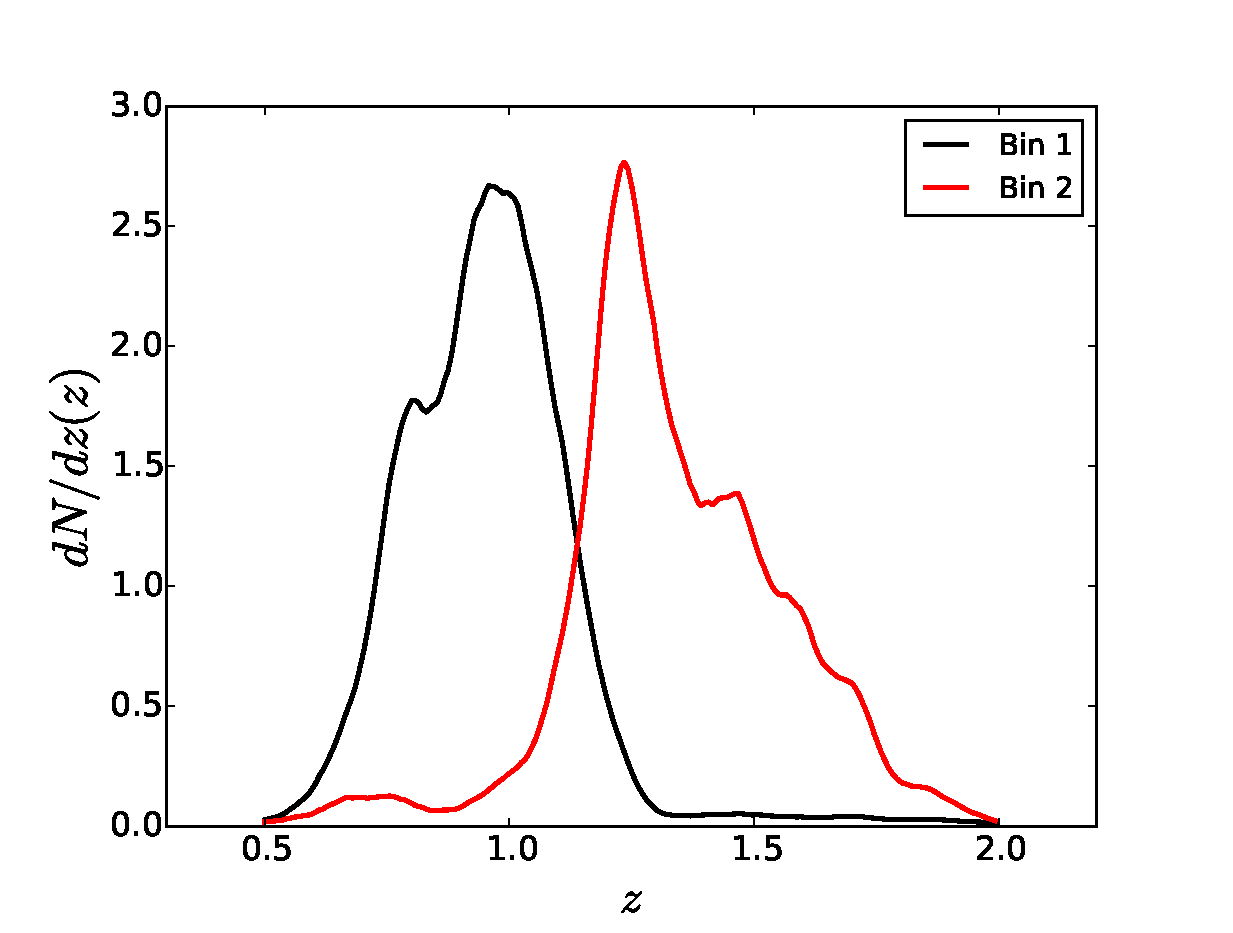
\includegraphics[width=0.6\textwidth]{zdist.eps}
\caption{Binned redshift distributions used for code comparison project.}
\label{fig:zhistos}
\end{figure}
%------------------------

In this second step, only 2 codes have been compared so far. More outputs are needed to guarantee convergence. Preliminarily, from these outputs, we have concluded that:
\begin{itemize}
\item The cross-correlation between bins is particularly sensitive to having enough points to sample the lensing kernel.
\item The nonlinear behaviour is sensitive to $l_{\rm max}$, we had to go up to 30,000 to get convergence (and we could not achieve $0.01\%$ convergence).
\item The large scales are sensitive to $l_{\rm min}$ (which also prompts a question about using the Limber approximation or not).
%\item Because we are using BBKS, evaluating the $P(k)$ at arbitrary $k_{\rm max}$ is not a problem, but we will need to test convergence in other cases.
\item The correlation functions are sensitive to how the power spectrum is interpolated. For example, in one case we had fewer $l$'s and we had to use an order $5$ spline. If we sample at all $l$'s then a linear interpolation is enough.
\end{itemize}

Additionally, independent codes were utilized to test the accuracy of halo mass function predictions. For the halo mass function, we compare the value of $\sigma$, $\log(\sigma^{-1})$, and the value of the halo mass function in the form used in \citep{Tinker2008},
\begin{equation}
\log[(M^2/\bar{\rho}_m)dn/dM].
\end{equation}
We note that while we maintain the $10^{-4}$ for our evaluations of $\sigma$, the accuracy degrades to a value of $5\times10^{-3}$ for the halo mass function evaluation, primarily at the high halo mass and high redshift domains. We find that this increased error is acceptable, as the level of precision is significantly better than the accuracy of current halo mass function models.

Finally, we note that formal tests for predictions in cosmologies with neutrinos are not yet included. The support for neutrino cosmologies in the current release is therefore not yet formally validated, although outputs have been informally compared against other codes where available. Formal validation of this functionality is ongoing.

{\tt CCL} has a suite of test routines which, upon compilation, compare its outputs to the benchmarks from code comparison. These are run with {\tt make check}.

\todo{What new checks were added?}

\todo{Add correlation function benchmarks (Elisabeth)}


\section{Default configuration}
\label{sec:default}

In its default configuration, {\tt CCL} adopts the nonlinear matter power spectrum from {\tt CLASS} through the Halofit implementation and the Tinker mass function for number counts.


\section{Examples for C implementation}
\label{sec:example}

Examples of how to run {\tt CCL} are provided in the {\tt tests} sub-directory of the library. The first resource for a new user should be the {\tt ccl$\_$sample$\_$run.c} file. This starts by setting up the {\tt CCL} default configuration. Then, it creates the ``cosmo'' structure, which contains distances and power spectra splines, for example. There are example calls for routines that output comoving radial distances, the scale factor, the growth factor and $\sigma_8$. Toy models are created for the redshift distributions of galaxies in the clustering and lensing samples, and for the bias of the clustering sample ($b(z)=1+z$). These are used for constructing the ``tracer'' structures via {\tt CCL$\_$Cltracer}, which can then be called to obtain the angular power spectra for clustering, cosmic shear and galaxy lensing.


\section{Python wrapper}
\label{sec:python}

A Python wrapper for {\tt CCL} is provided through a module called {\tt pyccl}. The whole {\tt CCL} interface can be accessed through regular Python functions and classes, with all of the computation happening in the background through the C code. The functions all support {\tt numpy} arrays as inputs and outputs, with any loops being performed in the C code for speed.

\subsection{Python installation}
\label{sec:python:install}

Before you can build the Python wrapper, you must have compiled and installed the C version of {\tt CCL}, as {\tt pyccl} will be dynamically linked to it. The Python wrapper's build tools currently assume that your C compiler is {\tt gcc} (with OpenMP enabled), and that you have a working Python 2.x installation with {\tt numpy} and {\tt distutils} with {\tt swig}. If you have installed CCL in your default library path, you can build and install the {\tt pyccl} module by going to the root {\tt CCL} directory and choosing one of the following options:
\begin{itemize}
 \item To build and install the wrapper for the current user only, run \\
 {\tt \$ python setup.py install --user}
 \item To build install the wrapper for all users, run \\
 {\tt \$ sudo python setup.py install}
 \item To build the wrapper in-place in the source directory (for testing), run \\
 {\tt \$ python setup.py build$\_$ext --inplace}
\end{itemize}
If you choose either of the first two options, the {\tt pyccl} module will be installed into a sensible location in your {\tt PYTHONPATH}, and so should be automatically picked up by your Python interpreter. You can then simply import the module using {\tt import pyccl}. If you use the last option, however, you must either start your interpreter from the root {\tt CCL} directory, or manually add the root {\tt CCL} directory to your {\tt PYTHONPATH}.

These options assume that the C library ({\tt libccl}) has been installed somewhere in the default library path. If this isn't the case, you will need to tell the Python build tools where to find the library. This can be achieved by running the following command first, before any of the commands above:

\texttt{python setup.py build$\_$ext --library-dirs=/path/to/lib/ --rpath=/path/to/lib/}

Here, {\tt /path/to/lib/} should point to the directory where you installed the C library. For example, if you ran {\tt ./configure --prefix=/my/path/} before you compiled the C library, the correct path would be {\tt /my/path/lib/}. The command above will build the Python wrapper in-place; you can then run one of the {\tt install} commands, as listed above, to actually install the wrapper. Note that the {\tt rpath} switch makes sure that the CCL C library can be found at runtime, even if it is not in the default library path. If you use this option, there should therefore be no need to modify the library path yourself.

On some systems, building or installing the Python wrapper fails with a message similar to:

\texttt{fatal error: `gsl/gsl$\_$interp2d.h' file not found.}

This happens when the build tools fail to find the directory containing the GSL header files, e.g. when they have been installed in a non-standard directory. To work around this problem, use the {\tt --include-dirs} option when running the {\tt setup.py build$\_$ext} step above, i.e. if the GSL header files are in the directory {\tt /path/to/include/}, you would run

\texttt{python setup.py build$\_$ext --library-dirs=/path/to/install/lib/ --rpath=/path/to/install/lib/ --include-dirs=/path/to/include/}

and then run one of the {\tt setup.py install} commands listed above. (Note: As an alternative to the {\tt --include-dirs} option, you can use {\tt -I/path/to/include} instead.)

You can quickly check whether {\tt pyccl} has been installed correctly by running {\tt python -c "import pyccl"} and checking that no errors are returned. For a more in-depth test to make sure everything is working, change to the {\tt tests/} sub-directory and run {\tt python run$\_$tests.py}. These tests will take a few minutes. Notice that these are not the same tests that are run via {\tt make check}. In the case of the {\tt python} tests, the library will only check for finite outputs of the routines called from {\tt pyccl}. There is no benchmark comparison in this case.
 
\subsection{Python example}
\label{sec:python:example}

The Python module has essentially the same functions as the C library, just presented in a more standard Python-like way. You can inspect the available functions and their arguments by using the built-in Python {\tt help()} function, as with any Python module.

Below is a simple example Python script that creates a new {\tt Cosmology} object, and then uses it to calculate the $C_\ell$'s for a simple lensing cross-correlation. It should take a few seconds on a typical laptop.

\begin{verbatim}
import pyccl as ccl
import numpy as np

# Create new Parameters object, containing cosmo parameter values
p = ccl.Parameters(Omega_c=0.27, Omega_b=0.045, h=0.67, A_s=2e-9, n_s=0.96)

# Create new Cosmology object with these parameters. This keeps track of
# previously-computed cosmological functions
cosmo = ccl.Cosmology(p)

# Define a simple binned galaxy number density curve as a function of redshift
z_n = np.linspace(0., 1., 200)
n = np.ones(z_n.shape)

# Create objects to represent tracers of the weak lensing signal with this
# number density (with has_intrinsic_alignment=False)
lens1 = ccl.ClTracerLensing(cosmo, False, z_n, n)
lens2 = ccl.ClTracerLensing(cosmo, False, z_n, n)

# Calculate the angular cross-spectrum of the two tracers as a function of ell
ell = np.arange(2, 10)
cls = ccl.angular_cl(cosmo, lens1, lens2, ell)
print cls
\end{verbatim}

Further examples are collected in several Jupyter notebooks available in the {\tt tests/} directory. These are:
\begin{verbatim}
Photo-z example.ipynb,

Power spectrum example.ipynb,

Distance Calculations Example.ipynb,

Lensing angular power spectrum.ipynb.
\end{verbatim}


\subsection{Technical notes on how the Python wrapper is implemented}
\label{sec:python:technical}

The Python wrapper is built using the {\tt swig} tool, which automatically scans the {\tt CCL} C headers and builds a matching interface in Python. The default autogenerated {\tt swig} interface can be accessed through the {\tt pyccl.lib} module if necessary. A more user-friendly wrapper has been written on top of this to provide more structure to the module, allow {\tt numpy} vectorization, and provide more natural Python objects to use (instead of opaque {\tt swig}-generated objects).

The key parts of the wrapper are as follows:
\paragraph{{\tt setup.py}} This instructs {\tt swig} and other build tools on how to find the right source files and set compile-time variables correctly. Most of this information is provided by header files and SWIG interface files that are included through the {\tt pyccl/ccl.i} interface file.

Note that certain compiler flags, like {\tt -fopenmp}, are also set in {\tt setup.py}. If you are not using {\tt gcc}, you may need to modify these flags (see the {\tt extra$\_$compile$\_$args} argument of the {\tt setup()} function).

\paragraph{Interface ({\tt .i}) files} These are kept in the {\tt pyccl/} directory, and tell {\tt swig} which functions to extract from the C headers. There are also commands in these files to generate basic function argument documentation, and remove the {\tt ccl$\_$} prefix from function names.

The interface files also contain code that tells {\tt swig} how to convert C array arguments to {\tt numpy} arrays. For certain functions, this code may also contain a simple loop to effectively vectorize the function.

The main interface file is {\tt pyccl/ccl.i}, which imports all of the other interface files. Most of the {\tt CCL} source files (e.g. {\tt core.c}) have their own interface file too. For other files, mostly containing support/utility functions, {\tt swig} only needs the C header ({\tt .h}) file to be specified in the main {\tt ccl.i} file, however. (The C source file must also be added to the list in {\tt setup.py} for it to be compiled successfully.)

\paragraph{Python module files} The structure of the Python module, as seen by the user, is organized through the {\tt pyccl/$\_$$\_$init$\_$$\_$.py} file, which imports only the parts of the {\tt swig} wrapper that are useful to the user. The complete autogenerated {\tt swig} interface can be accessed through the {\tt pyccl.lib} sub-module if necessary.

Individual sub-modules from {\tt CCL} are wrapped in their own Python scripts (e.g. {\tt power.py}), which typically provide a nicer ``Pythonic'' interface to the underlying {\tt CCL} functions and objects. This includes automatically choosing whether to use the vectorized C function or not, as well as some conversions from Python objects to the autogenerated {\tt swig} objects. Most of the core Python objects, like {\tt Parameters} and {\tt Cosmology}, are defined in {\tt core.py}. These objects also do some basic memory management, like calling the corresponding {\tt ccl$\_$free$\_$*} C function when the Python object is destroyed.

\paragraph{Auto-generated wrapper files} The {\tt swig} command is triggered when you run {\tt setup.py}, and automatically generates a number of C and Python wrapper files in the {\tt pyccl/} directory. These typically have names like {\tt ccl$\_$*.c} and {\tt ccl$\_$*.py}, and should not be edited directly, as {\tt swig} will overwrite them when it next runs.

\paragraph{{\tt pyccl/pyutils.py}} This file contains several generic helper functions for passing {\tt numpy} arrays in and out of Python functions in a convenient way, and for performing error checking and some type conversions.

The build process will also create a {\tt pyccl/ccllib.py} file, which is the raw autogenerated Python interface, and {\tt $\_$ccllib.so}, which is a C library containing all of the C functions and their Python bindings. A {\tt build/} directory and {\tt pyccl.egg-info/} directory will also be created in the same directory as {\tt setup.py} when you compile {\tt pyccl}. These (plus the {\tt pyccl/$\_$ccllib.so} file) should be removed if you want to do a clean recompilation. Running {\tt python setup.py clean --all} will remove some, but not all, of the generated files.


\section{Future functionality to be included}
\label{sec:future}

In the future, we hope that {\tt CCL} will include other functionalities. Functionalities which are currently under development:
\begin{itemize}
	\item a link to FAST-PT \citep{FASTPT} for implementation of perturbation theory,
	\item a more realistic photo-z model,
	\item support for cosmologies with multiple unequal-mass neutrinos,
	\item and more power spectrum methods (see \ref{Pk_whishlist}).
\end{itemize}

\section{Feedback}
\label{sec:feedback}

If you would like to contribute to {\tt CCL} or contact the developers, please do so through the {\tt CCL} github repository located in \url{https://github.com/LSSTDESC/CCL}.

\section{License}
\label{sec:license}

Copyright \textcopyright 2017, the LSSTDESC CCL contributors are listed in the
documentation (``research note'') provided with this software. The repository can be found at \url{https://github.com/LSSTDESC/CCL}. All rights reserved.

Redistribution and use in source and binary forms, with or without
modification, are permitted provided that the following conditions are met:

\begin{itemize}
\item Redistributions of source code must retain the above copyright notice, this
  list of conditions and the following disclaimer.
\item Redistributions in binary form must reproduce the above copyright notice,
  this list of conditions and the following disclaimer in the documentation
  and/or other materials provided with the distribution.
\item Neither the name of CCL (\url{https://github.com/LSSTDESC/CCL}) nor the names of its
  contributors may be used to endorse or promote products derived from
  this software without specific prior written permission.
\end{itemize}

THIS SOFTWARE IS PROVIDED BY THE COPYRIGHT HOLDERS AND CONTRIBUTORS ``AS IS''
AND ANY EXPRESS OR IMPLIED WARRANTIES, INCLUDING, BUT NOT LIMITED TO, THE
IMPLIED WARRANTIES OF MERCHANTABILITY AND FITNESS FOR A PARTICULAR PURPOSE ARE
DISCLAIMED. IN NO EVENT SHALL THE COPYRIGHT HOLDER OR CONTRIBUTORS BE LIABLE
FOR ANY DIRECT, INDIRECT, INCIDENTAL, SPECIAL, EXEMPLARY, OR CONSEQUENTIAL
DAMAGES (INCLUDING, BUT NOT LIMITED TO, PROCUREMENT OF SUBSTITUTE GOODS OR
SERVICES; LOSS OF USE, DATA, OR PROFITS; OR BUSINESS INTERRUPTION) HOWEVER
CAUSED AND ON ANY THEORY OF LIABILITY, WHETHER IN CONTRACT, STRICT LIABILITY,
OR TORT (INCLUDING NEGLIGENCE OR OTHERWISE) ARISING IN ANY WAY OUT OF THE USE
OF THIS SOFTWARE, EVEN IF ADVISED OF THE POSSIBILITY OF SUCH DAMAGE.

Contact GitHub API Training Shop Blog About \textcopyright 2017 GitHub, Inc. Terms Privacy Security Status Help

%
This paper has undergone internal review in the LSST Dark Energy Science Collaboration. We thank the reviewers: Mike Jarvis, Yao-Yuan Mao and Mariana Penna-Lima for comments that helped improved this manuscript and the \ccl library overall. We thank Matt Becker for helping us address the \ccl code review.

%DESC standard paper acknowledgements
%From https://github.com/LSSTDESC/desc-tex/blob/master/ack/standard.tex
The DESC acknowledges ongoing support from the Institut National de Physique Nucl\'eaire et de Physique des Particules in France; the Science \& Technology Facilities Council in the United Kingdom; and the Department of Energy, the National Science Foundation, and the LSST Corporation in the United States.  DESC uses resources of the IN2P3 Computing Center (CC-IN2P3--Lyon/Villeurbanne - France) funded by the Centre National de la Recherche Scientifique; the National Energy Research Scientific Computing Center, a DOE Office of Science User Facility supported by the Office of Science of the U.S.\ Department of Energy under Contract No.\ DE-AC02-05CH11231; STFC DiRAC HPC Facilities, funded by UK BIS National E-infrastructure capital grants; and the UK particle physics grid, supported by the GridPP Collaboration. This work was performed in part under DOE Contract DE-AC02-76SF00515. 

%In addition
We would like to thank the organisers of the DESC meetings and hack weeks in the period 2015-2018, where this work was partly developed. We would also like to acknowledge the contribution of the participants of the Theory and Joint Probes Code Comparison Project, some of whom are among the \ccl contributors, for providing the benchmarks for testing CCL. We also acknowledge Louis Penafiel and Elizabeth Kimura, who developed the {\tt VARRIC} code to compare and visualize power spectra calculated by \ccl and {\tt CLASS}. We thank Pedro Ferreira for feedback on this manuscript. We are grateful for the feedback received from other working groups of DESC, including Strong Lensing, Supernovae, Clusters and Photometric Redshifts. We are grateful to Katrin Heitmann and Earl Lawerence for discussions concerning the Cosmic Emulator. We are also thankful to the {\tt CLASS} authors and to Andrew Hamilton for making their codes available and allowing us to use them in this work. We thank Peter Williams for making his ApJ bibstyle file available\footnote{\url{https://github.com/pkgw/tex-stuff/blob/master/yahapj.bst}.}.  
%

DA is supported by the Science and Technology Facilities Council (STFC) through an Ernest Rutherford Fellowship, grant reference ST/P004474/1. NEC acknowledges support from a Beecroft fellowship and a Royal Astronomical Society Research Fellowship. TT acknowledges funding from the European Union's Horizon 2020 research and innovation programme under the Marie Sk{l}odowska-Curie grant agreement No.\ 797794. MI acknowledges that this material is based upon work supported in part by NSF under grant AST-1517768 and the U.S. Department of Energy, Office of Science, under Award Number DE-SC0019206.


Author contributions are listed below. \\
Husni Almoubayyed: Reviewed code/contributed to issues. \\
David Alonso: Co-led project; developed structure for angular power spectra; implemented autotools; integrated into LSS pipeline; contributed to: background, power spectrum, mass function, documentation and benchmarks; reviewed code \\
Jonathan Blazek: Planning capabilities and structure; documentation and testing. \\
Philip Bull: Implemented the Python wrapper and wrote documentation for it; general bug fixes, maintenance, and code review; enhanced the installer and error handling system. \\
Jean-\'Eric Campagne: Angpow builder and contributed to the interface with CCL. \\
N. Elisa Chisari: Co-led project, coordinated hack projects \& communication, contributed to: correlation function \& power spectrum implementation, documentation, and comparisons with benchmarks. \\
Alex Drlica-Wagner: Helped with document preparation. \\
Tim Eifler: Reviewed/tested code. \\
Ren\'ee Hlozek: Contributed initial code for error handling structures, reviewed other code edits. \\
Mustapha Ishak: Contributed to planning of code capabilities and structure; reviewed code; identified and fixed bugs. \\
David Kirkby: Writing, testing and reviewing code. Asking questions. \\
Elisabeth Krause: Initiated and co-led project; developed CLASS interface and error handling; contributed to other code; reviewed pull requests. \\
C. Danielle Leonard: Wrote and tested code for LSST specifications, user-defined photo-z interface, and support of neutrinos; reviewed other code; wrote text for this note. \\
Phil Marshall: Helped with document preparation. \\
Thomas McClintock: Wrote Python documentation. \\
Sean McLaughlin: Wrote doxygen documentation and fixed bugs/added functionality to distances. \\
J\'er\'emy Neveu: Contributed to Angpow and built the interface with CCL. \\
St\'ephane Plaszczynski: Contributed to Angpow and contributed to the interface with CCL. \\
Javier Sanchez: Modified setup.py to allow pip installation and uninstall. \\
Sukhdeep Singh: Contributed to the correlation functions code. \\
An\v{z}e Slosar: Wrote and reviewed code. \\
Antonio Villarreal: Contributed to initial benchmarking, halo mass function code, and general code and issues review. \\
Michal Vrastil: Wrote documentation and example code, reviewed code. \\
Joe Zuntz: Wrote initial infrastructure, C testing setup, and reviewed code. \\



%{\it Facilities:} \facility{LSST}

\bibliography{main}

\end{document}
%
